\documentclass[PICOAPC.tex]{subfiles}
\newcommand\pdeg{.\!\!\degree}
\newcommand\parcm{.\!\!'}


\section{Schedule and Cost}
\label{sec:mission_schedule}

%\subsection{Schedule}
%\label{sec:mission_schedule}

\vspace{-0.1in}
\begin{figure}[hb]
\begin{center}
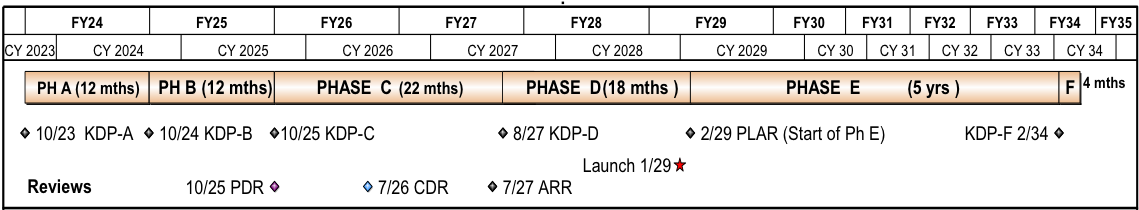
\includegraphics[width=\textwidth]{figures/Schedule.png}
\end{center}
\vspace{-0.30in}
\caption{\captiontext PICO development and operations schedule. \label{fig:Schedule}}
\vspace{-0.05in}
\end{figure}

$\bullet$ {\bf Schedule} \hspace{0.1in} NASA-funded Probe studies including PICO assume a Phase~A start in October 2023. PICO development phases B-D are similar in duration to recent comparably sized NASA missions such as Juno and SMAP. PICO is a cryogenic mission similar to \planck , but the cryogenic design is simpler because all PICO's bolometric detectors are maintained at 0.1~K (\planck 's bolometers were maintained at 0.1~K, and the radiometers at 20~K).  We used experience from \planck\ and from current implementations of ground-based kilo-pixel arrays  to allocate appropriate time for integration and testing (I\&T). 

The baseline mission lifetime is 5 years. The PICO instrument does not have cryogenic consumables (as Planck did), permitting mission extension beyond the prime mission duration. 

\input tables/table-cost.tex
$\bullet$ {\bf Cost} \hspace{0.1in}  We estimate PICO's total Phase A--E lifecycle cost between \$870M and \$960M, including the \$150M allocation for the Launch Vehicle (per NASA direction). These cost estimates include 30\,\% reserves for development (Phases A--D) and 13\,\% reserves for operations (Phase~E). Table~\ref{tab:cost} shows the 
JPL Team~X and the PICO team mission cost breakdown. Team~X estimates are generally model-based, and were generated after a series of instrument and mission-level studies. The PICO team adopted the Team~X estimates, but also obtained a parametrically estimated cost range for the Flight System and Assembly, Test, and Launch Operations from Lockheed Martin Corporation to represent the cost benefits that might be realized by working with an industry partner. After adding estimated JPL overhead 
%and Team~X estimated V-groove assembly costs (not included in the Lockheed estimate), 
the PICO team cost is in-family with but lower than the Team~X cost.

Science team costs are assessed by Team~X based on PICO science team estimates of the numbers and types of contributors and meetings required for each year of PICO mission development and operations. These workforce estimates are informed by recent experience with the \planck\ mission. PICO's spacecraft cost reflects a robust Class~B architecture. Mission-critical elements are redundant. Appropriate flight spares, engineering models and prototypes are included. Mission operations, Ground Data Systems, and Mission Navigation and Design costs reflect the relatively simple operations: PICO has a single instrument and a single, repetitive science observing mode. 

The active cooling system (the 0.1\,K cADR and 4\,K cryocooler) comprises nearly half of the payload cost. The cADR cost for this study is an estimate from Goddard Space Flight Center. The 4\,K cryocooler cost for this study is based on the NASA Instrument Cost Model (NICM) VIII CER Cryocooler model
\cite{Mrozinski2017}, assuming a commercial build. Based on JPL experience, 18\,\% of the instrument cost is allocated for integration and testing (I\&T). More details on the cost of PICO are available in the full PICO report~\citep{pico_report}.

%\subsection{Heritage}
%\label{sec:heritage} %6.3

%PICO's reflectors are similar to \planck 's, but somewhat larger ($270 \,\, {\rm cm} \times 205\,{\rm cm}$ primary versus $189\,{\rm cm} \times 155\,{\rm cm}$)~\citep{Gloesener2006}. \textit{Herschel} observed at shorter wavelengths that required higher surface accuracy and had a larger reflector ($350\, \,{\rm cm}$ diameter primary)~\citep{Toulemont2004}. PICO's detectors are cooled by a cADR with requirements that are within the capabilities of current ADRs developed by Goddard Space Flight Center. These systems have been applied to several JAXA missions, including \textit{Hitomi}~\citep{Shirron2016}. PICO's 4\,K cryocooler (\S\,\ref{sec:4kcooler}) is a direct extension of the JWST MIRI design~\citep{Durand2008,Rabb2013}. PICO benefits from a simpler and more reliable implementation of the J-T system than was required for MIRI, in that no deployment of cooling lines is required, and all flow valving is performed on the warm spacecraft. Structures similar to PICO's V-groove radiator assembly are a standard approach for passive cooling, and were first described more than thirty years ago~\citep{Bard1987}. PICO's spin system is less demanding than the successful SMAP spin system. The PICO spin rate is 1\,rpm, and the mission requires $\sim220$\,N\,m\,s of spin angular momentum cancellation. The PICO's data volume and downlink rates are already surpassed by missions in development. 

%\end{document}

